%pandoc -f latex -t docx  geospatial-stroke.tex --bibliography references.bib -o geospatial.docx --csl=frontiers-in-physics.csl
\documentclass[utf8]{frontiersHLTH}

\usepackage{url,hyperref,lineno,microtype,subcaption}
\usepackage[onehalfspacing]{setspace}
\usepackage{verbatimbox}
\usepackage{mdframed}
\usepackage{color}
\definecolor{dkgreen}{rgb}{0,0.6,0}
\definecolor{gray}{rgb}{0.5,0.5,0.5}
\definecolor{mauve}{rgb}{0.58,0,0.82}
\usepackage{listings}
\lstset{language=R,
basicstyle=\footnotesize,       % the size of the fonts that are used for the code
  numbers=left,                   % where to put the line-numbers
  numberstyle=\tiny\color{gray},  % the style that is used for the line-numbers
  stepnumber=1,                   % the step between two line-numbers. If it's 1, each line
                                  % will be numbered
  numbersep=5pt,                  % how far the line-numbers are from the code
  backgroundcolor=\color{white},  % choose the background color. You must add \usepackage{color}
  showspaces=false,               % show spaces adding particular underscores
  showstringspaces=false,         % underline spaces within strings
  showtabs=false,                 % show tabs within strings adding particular underscores
  frame=single,                   % adds a frame around the code
  rulecolor=\color{black},        % if not set, the frame-color may be changed on line-breaks within not-black text (e.g. commens (green here))
  tabsize=2,                      % sets default tabsize to 2 spaces
  captionpos=b,                   % sets the caption-position to bottom
  breaklines=true,                % sets automatic line breaking
  breakatwhitespace=false,        % sets if automatic breaks should only happen at whitespace
  %keywordstyle=\color{blue},      % keyword style
  keywordstyle=\ttfamily,
  commentstyle=\color{dkgreen},   % comment style
  stringstyle=\color{mauve},      % string literal style
  escapeinside={\%*}{*)},         % if you want to add a comment within your code
  deletekeywords={transform,set,distance,mode,count,as,by,read,csv},
  morekeywords={}            % if you want to add more keywords to the set}
}
\linenumbers

\def\keyFont{\fontsize{8}{11}\helveticabold }
\def\firstAuthorLast{Padgham {et~al.}} %use et al only if is more than 1 author
\def\Authors{Mark Padgham\,$^{1}$, Geoff Boeing\,$^{2}$, David Cooley\,$^{3}$, Nicholas Tierney\,$^{4}$, Michael Sumner\,$^{5}$, Thanh G Phan\,$^{7,8}$ and Richard Beare\,$^{9,10,*}$}
% Affiliations should be keyed to the author's name with superscript numbers and be listed as follows: Laboratory, Institute, Department, Organization, City, State abbreviation (USA, Canada, Australia), and Country (without detailed address information such as city zip codes or street names).
% If one of the authors has a change of address, list the new address below the correspondence details using a superscript symbol and use the same symbol to indicate the author in the author list.
\def\Address{$^{1}$Active Transport Futures, Muenster, Germany\\
$^{2}$School of Public Policy and Urban Affairs, Northeastern University, Boston, Massachusetts, USA\\
$^{3}$Symbolix Pty Ltd, Melbourne, Victoria, Australia \\
$^{4}$Department of Econometrics and Business Statistics, Monash University, Melbourne, Victoria, Australia\\
$^{5}$Australian Antarctic Division, Department of the Environment and Energy, Kingston, Tasmania, Australia\\
$^{7}$Clinical Trials Imaging and Informatics Division of Stroke and Aging Research Group, Monash University, Melbourne, Victoria, Australia\\
$^{8}$Stroke Unit, Monash Medical Centre, Melbourne, Victoria, Australia\\
$^{9}$Department of Medicine, Monash University, Melbourne, Victoria, Australia\\
$^{10}$Developmental Imaging, Murdoch Children's Research Institute, Melbourne, Victoria, Australia}

% The Corresponding Author should be marked with an asterisk
% Provide the exact contact address (this time including street name and city zip code) and email of the corresponding author
\def\corrAuthor{Richard Beare\\Peninsula Clinical School\\Frankston Hospital\\2 Hastings Rd\\Frankston\\Victoria 3199\\Australia}

\def\corrEmail{Richard.Beare@monash.edu}

\begin{document}
\onecolumn
\firstpage{1}

\title[Software tools for geospatial analysis]{{\bf An Introduction to} software tools, data and services for geospatial analysis of stroke services}

\author[\firstAuthorLast ]{\Authors} %This field will be automatically populated
\address{} %This field will be automatically populated
\correspondance{} %This field will be automatically populated

\extraAuth{}% If there are more than 1 corresponding author, comment this line and uncomment the next one.
%\extraAuth{corresponding Author2 \\ Laboratory X2, Institute X2, Department X2, Organization X2, Street X2, City X2 , State XX2 (only USA, Canada and Australia), Zip Code2, X2 Country X2, email2@uni2.edu}

\maketitle

\begin{abstract}
  {\bf
Background: There are interests in the use geospatial data for
development of acute stroke services given the importance of timely acess
to acute reperfusion therapy. This paper aims to introduce clinicians and
citizen scientists to the possibilities offered by open source softwares (R
and Python) for analyzing geospatial data. It is hope that this introduction
would stimulate interest in the field as well as generate ideas for improving
stroke services.

Method: Instructions on installation of libraries for R and Python, source
codes and links to census data are provided in a notebook format to
enhance experience with running these softwares. These codes illustrate
different aspects of using geospatial analysis: 1)- creation of choropleth
(thematic) map which depicts estimate of stroke cases per post codes; 2)
use of map to help define service regions for rehabilitation after stroke.

Results: Choropleth map showing estimate of stroke per post codes and
service boundary map for rehabilitation after stroke.
Conclusions The examples in this article illustrate the use of a range of
components that underpin geospatial analysis. By providing an accessible
introduction to these areas, clinicians and researchers can create code to
answer clinically relevant questions on topics such as service delivery
and service demand.
}
\end{abstract}
\section{Introduction}\label{introduction}

{\bf
  Endovascular clot retrieval (ECR) and thrombolysis enables reperfusion
following ischemic stroke and results in dramatic reversal of
neurological deficit in selected patients
\cite{berkhemer2015randomized,goyal2016endovascular,goyal2015randomized,campbell2015endovascular,saver2015stent,ma2019thrombolysis}.
The publication of the DEFUSE3 (Endovascular Therapy Following Imaging
Evaluation for Ischemic Stroke) and DAWN (DWI or CTP Assessment with
Clinical Mismatch in the Triage of Wake-Up and Late Presenting Strokes
Undergoing Neurointervention with Trevo) trials potentially pushed the
boundary for performing ECR in a small set of patients to 24
hours\cite{nogueira2018thrombectomy,albers2018thrombectomy} and
thrombolysis to 9 hours \cite{ma2019thrombolysis}. ECR treatment requires
specialist centers with 24-hour staffing by skilled stroke teams and
interventional radiologists with unrestricted access to angiography
suites. Key decisions for governments and policy makers include: how
many centers are required to service a specified area, how to identify
redundant centres, where should
the centers be placed and what is the expected load on the
centers\cite{Phan_2017}. Many factors influence the final choice,
including the availability of trained interventional neuroradiologists
(INR), the number of cases required for INR to retain skills, and
costs.


Related to the above considerations is the issue of transport
model. One proposed model is direct transport to mothership (ECR hub)
whereby ambulance bypass the smaller hospitals including those which
are thrombolysis capable and take the patient to directly to the ECR
hub \cite{Milne_2017, 10.1001/jamaneurol.2018.2424}. The alternative
model is the ``drip and ship'' model whereby patients are brought to
the nearest thrombolysis centre for advanced imaging and triaging on
the need for thrombolytic drug and or ECR. A drawback to the drip and
ship model is that there is an additional 99 minutes delay related to
a second transfer of the case with large vessel occlusion (LVO) to the
mothership\cite{froehler2017interhospital}. Investigators recently
proposed inclusion of speed of delivery of thrombolysis as an additional
consideration \cite{10.1001/jamaneurol.2018.2424}. Identification of patients
for ECR at the pre-hospital level requires either the use of LVO scale
or mobile stroke unit (MSU). Before LVO scales can be used in the
field, the impact from its use on ECR hub loading (handling of large
volume of ECR and non-ECR cases) has to be tested.

In the writing of this introduction, we have asked several data
scientists (software engineers) to contribute the introduction to
geospatial analysis for clinicians and other citizen scientists
aspiring to work in the field. Alternatively, a deeper understanding
of these geospatial methods will enable clinicians to collaborate with
other researchers or citizen scientists on models to improve local
stroke service. Both codes and data are provided so that once {\em R} and
{\em Python} softwares are installed, the scientist can copy and paste the
example codes to test run. These softwares typically involve
relatively steep learning curves and as such instructions for running
the softwares are provided; please see the more extensive codes and
data on our github address \href{https://richardbeare.github.io/GeospatialStroke/}{https://richardbeare.github.io/GeospatialStroke/}).
The examples provided here are not exhaustive and are
intended to stimulate creative use of these geospatial tools. The two
examples we present are a choropleth (thematic map) and a service
catchment basin estimation. A choropleth is a thematic map display in
which regions are coloured by a measure of the region. We use
demographic and boundary data from the Australian Bureau of Statistics
and incidence data from the NEMESIS
\cite{thrift_stroke_2000,azarpazhooh2008patterns} study to estimate
stroke cases per postcode and display the result on an interactive
map. The service catchment basin estimation involves a Monte-Carlo
simulation of patients attending a rehabilitation service of 3
hospitals. The catchment basin of each hospital is the region that has
lower travel time to that hospital than any other. Catchment basins
can be combined with incidence data to estimate load on rehabilitation
centers. The data can be used to explore scenarios, such as the
removal or addition of service centers.
}
%Geospatial approaches have been used to %analyse the delivery of
%emergency clot retrieval services %\cite{Phan_2017} and to evaluate
%``Drip and Ship'' approaches in %specific locales \cite{Milne_2017}
%and population level %access to services
%\cite{Adeoye_2014}. %Geospatial tools can be used to analyse and
%visualise geospatial data, %such as patient collection location as
%well as perform a range of %simulations at varying levels of
%detail. For example, in %\cite{Phan_2017}, travel times between a set
%of randomly generated %addresses and a set of possible destinations
%were estimated using %queries to several Google Application
%Programming Interfaces (API), %allowing various configuration of the
%treatment network to be %tested. Combination of the resulting
%catchment areas with demographic %data allowed loadings to be
%estimated. %The studies cited above were constructed using a series
%of standard %geospatial analysis components. In this article we will
%introduce %these components and provide examples of how they can be
%used to %answer health related questions. Examples are implemented
%using open %source software, specifically R and Python, and source
%code provided %so that readers can reproduce and modify them
%%\cite{R_Core_Team_2018,sanner1999python,boeing_osmnx_2017}. Geospatial
%analysis tools %have traditionally been the domain of specialist
%commercial software %and vendors, however this is no longer the case,
%with a range of open %source options available to researchers. These
%tools are extremely %flexible, but typically involve relatively steep
%learning curves. We %hope that his article will provide stroke
%researchers with a useful %introduction to the possibilities offered
%by these tools.

\section{Geospatial Analysis}\label{background} 
{\bf
{\em Geospatial analysis} or modelling of spatial data has
traditionally been the domain of {\em geographic information systems
  (GIS)} specialists, employing commercial software and data
products. Recent years, however, have seen the development of open
source tools and free or low cost web services, such as Google Maps,
that make geospatial analysis accessible and feasible to the
non-specialist citizen scientist. In this article we introduce a
family of computational techniques and services, collectively termed
geospatial analysis tools, that can be applied to a range of questions
relevant to stroke services. The codes used here are for two free
and open source software environments - {\em R} and  {\em Python}. Geospatial analysis
can also be performed with Matlab\cite{Milne_2017}; this software is not free and
will not be discussed further. Geospatial analysis tools allow
manipulation and modelling of geospatial data. These tools, data, and
modelling techniques have a long track record in the quantitative
geography, city and regional planning, and civil engineering research
literatures. Geospatial data, in the context of stroke research,
includes the location of patients and treatment centers, routes
through the road network linking patients to treatment centers,
geographic and administrative region boundaries (e.g.~post codes,
government areas, national boundaries) and disease incidence and
demographic information associated with such regions.
}
\subsection{Geospatial frameworks}\label{geospatial-frameworks} 
In geospatial analysis, the location of a data point on the Earth's surface is referred
to in terms of longitude and latitude. In practice, longitude is the X
axis and latitude is the Y axis. More complex data, such as national
boundaries or administrative or postcode boundaries consist of sets of
points connected together in defined orders, typically to produce a
closed shape. Other structures, such as road networks, are also
constructed using sets of points and include other types of
information, such as speed limits, travel direction etc. A geospatial
framework provides mechanisms for representing, loading, and saving
geospatial data and performing fundamental mathematical
operations. For example, the simple features (sf) \cite{Pebesma_2018}
package, on which our R examples are based, provides structures to
represent all manner of shapes and associate them with non-spatial
quantities, perform transforms between coordinate systems, display
shapes, compute geometric quantities like areas and distances and
perform operations like intersections and unions. The equivalent
Python framework is the geopandas package that provides a geospatial
extension to standard data frames. A key emerging subdomain of
geospatial analysis is spatial network analysis. Several open-source
packages now exist for modelling and analyzing spatial networks, such
as urban street networks, including dodgr for R \cite{Padgham_2019}
and OSMnx for Python \cite{boeing_osmnx_2017}.

\subsection{Sources of regional data}\label{sources-of-regional-data} 

The examples below use postcode boundary data available from the
Australian Bureau of Statistics (the codes for performing this task
are available in the supplementary material or on the website
\href{https://richardbeare.github.io/GeospatialStroke/}{https://richardbeare.github.io/GeospatialStroke/}). It
is common for boundaries used in reporting of regional statistics to
be available in standard file formats from the reporting bodies or
central authorities along with the reported statistics. The regional
demographics measures, often derived from national census data, also
represent an important source of information for researchers,
including age, sex, income, ethnicity etc. For example, in the US, key
data sources on sociodemographics and the built environment include
the Census Bureau's decennial census \cite{us_census_bureau_decennial}
(a complete enumeration at fine spatial scales but coarse, decadal
temporal scales), American Community Survey\cite{us_census_bureau_acs}
(a survey with annual temporal scales, but often fairly large standard
errors at small spatial scales due to the sample size), and TIGER/Line
shapefiles\cite{us_census_tiger_line} of tract, municipal, and
urbanized area boundaries. A comprehensive repository of US road
network models at regional and municipal scales is available on the
Harvard Dataverse \cite{boeing_street_2019}. Additional regional data
are frequently available from municipal, state, county, or
metropolitan governmental agencies. Demographic data for countries in
the European Union are provided by Eurostat \cite{eurostat}. This
includes time series data from several years to decades on economics,
demography, infrastructure, health, traffic, and more of the EU
\cite{Lahti2017}. Geographic data for the EU is available through the
Geographic Information System of the COmmission (GISCO), part of
Eurostat. Similar levels of demographic data are available from France
through INSEE \cite{insee}, Germany through Destatis \cite{destatis}
and, Switzerland through \cite{swiss-bfs}. There are a number of
European sources of geospatial data \cite{diva-gis,germany-gis,swiss-3d}.

\subsection{Geocoding and reverse geocoding}\label{geocoding-and-reverse-geocoding} 

Location information, such as a patient's home address, is often
available as a street address, rather than coordinates (a
longitude/latitude pair). However, operations such as plotting
addresses on a map require coordinates. Geocoding is the process of
converting an address to a coordinate pair. Reverse geocoding converts a
coordinate pair to an address. Coordinates are useful in many other types
of computation, as we shall see in the examples below. There are two
common approaches to geocoding and reverse geocoding. The most
ubiquitous is via web services such as Google Maps. Other services,
such as OpenStreetMap's Nominatim web service and OpenCage
(\url{https://opencagedata.com/}), provide similar capabilities and
all can be queried in an automated way from R and Python
\cite{opencage}. The other approach is via a local database of
geocoded addresses. One example, for Australia, is the PSMA (formerly
Public Sector Mapping Agencies) address database available in an R
queryable form. A local database allows many high speed queries, but
is often less flexible in terms of query structure than the web
services. Web services are discussed in more detail below.

\subsection{Distance and travel {\bf time} estimation}\label{distance-and-travel-estimation} 

A key part of a number of studies cited above is the estimation of
travel time between patient and treatment center. The popularity of
personal navigation systems in smartphones has driven the development
of extremely sophisticated tools to estimate the fastest route between
points. One of the best known, Google Maps \footnote{the two APIs
  involved are the directions api and distance api}, uses a
combination of information about the road network, historic travel
time data derived from smartphone users and live information from
smartphones. The travel time estimates are thus sensitive to time of
day, weather conditions and possibly traffic accidents. Google, and
other web services for travel time estimation, can be queried in a
similar fashion to the geocoding services. It is also possible to
create a local database to represent the road network, allowing more
rapid querying, but losing some of the benefits of traffic models.

\subsection{Visualization}\label{visualization} 

Two forms of visualization are used in the following examples - static
and interactive. Static maps are required for printed reports and
typically present a carefully selected view. Interactive maps allow
exploration of a data set, via zooming and toggling of
overlays. Interactive maps often use web services to provide the
background map ``tiles'', over which data is superimposed. Different
interactive web services specialise in different types of
display. Some tools produce static and interactive displays in very
similar ways.

\subsection{Introduction to web services}\label{introduction-to-web-services}

Web services providing various forms of geospatial capabilities are a
crucial component of the geospatial analysis tools now available to
researchers. Web services deliver what used to be complex and
specialised information products to the general public. Geocoding and
travel time estimation are two common examples that have already been
discussed. Other capabilities include delivery of tiled maps (such as
the Google Maps display), street network and building footprint data
(such as from OpenStreetMap), and census data on sociodemographic or
built environment characteristics (such as from the US Census Bureau).

\subsubsection{Application programming interfaces (API)}\label{application-programming-interfaces-api} 
Web services such as Google Maps are accessible via an API. The API
allows software tools, such as {\em R} or {\em Python}, to make
requests to the web service and retrieve results. Thus, if we consider
the Google Maps example, not only can a user access a map query for an
address via a web browser, but a program can submit the same
request. Furthermore, a program can submit a series of automated
requests. For example, given a list of addresses, it is relatively
simple to generate an R or Python procedure to geocode all of them via
a web service. Many APIs such as Google Maps are commercial products
and thus charge for use, although the use is often free for small
volumes (typical limit is 2500 queries per day). The combination of
these factors tends to mean that many APIs require somewhat complex
setup, typically via signup and creation of keys. Terms of use may
evolve over time, with charging being introduced, possibly leading to
a need to enter credit card details (necessary for Google Maps API). We have endeavoured to create
examples that do not require keys, simplifying getting
started (tmaptools and OpenStreetMap). However, some extensions have been included that do require
keys. These are described in supplementary material.

\subsubsection{OpenStreetMap (OSM)}\label{openstreetmap-osm} 
OSM (\url{https://www.openstreetmap.org/}) is a service collecting and
distributing crowdsourced geospatial data. Many useful OSM services
are available without API keys, and it is thus the platform of choice
for examples in this paper. OSM is also unusual in that it allows
access to underlying geospatial structures, such as road networks, rather than
images generated from those structures. This capability is used to
estimate travel time.

\subsubsection{Access to the examples}\label{access-to-the-examples} 
The examples are available in their source code form from
\url{https://github.com/richardbeare/GeospatialStroke/archive/master.zip}. ``Live''
versions and instructions are available at
\url{https://richardbeare.github.io/GeospatialStroke/index.html}
and can be viewed in conjunction with the methods section. The
description focuses on the {\em R} versions of the examples. Code is
visible in the shaded boxes, while output of the code, such as maps,
are displayed immediately after the code. {\em Python} versions are
provided and implement equivalent steps. Details on downloading and
running the examples are available in supplementary material and at
the web site.

\section{Methods}\label{methods}
{\bf
The key sections of code used in the methods are presented and
described in tables in this article. These pieces of code are not
intended to be executed in isolation, and are best appreciated in the
complete examples (both code and data), which are too long to include
directly in the article, but are available for download, as described
in Section \ref{access-to-the-examples}.
}
\subsection{Example 1: Choropleth to visualize estimated stroke numbers}\label{example-1-choropleth-to-visualize-estimated-stroke-numbers} 

\subsubsection{Overview:}\label{overview} 
We demonstrate accessing and using different data sources. The first
is Australian Bureau of Statistics census data provided at the
postcode level for population information, stratified by age, as well
as postcode boundary information. The second data source is incidence
data from the North East Melbourne Stroke Incidence Study
(NEMESIS)\cite{thrift_stroke_2000}. This is combined with the first
dataset to estimate per-postcode stroke incidence. We demonstrate
geocoding by finding the location of a hospital delivering acute
stroke services, and then display postcodes within 15km, colouring
each postcode by estimated stroke incidence. The steps involved are
described in Tables \ref{tab:exampleA1} and \ref{tab:exampleA2}.

\subsubsection{Example 2: Service regions for stroke rehabilitation}\label{example-2-service-regions-for-stroke-rehabilitation} 
In the second example we demonstrate the idea of estimating catchment
basins for a set of three service centers (network comprising three
rehabilitation hospitals servicing a hospital with an acute stroke
service). The idea can be easily extended to more service centers. A
catchment basin, or catchment area for a service center is the region
that is closer to that service center than any other. The definition
of ``closer'' is critical in this calculation, with travel time
through the road network being a useful measure for many practical
purposes. The approach used in this example involves the sampling of
random addresses within a region of interest around the service
centers, estimation of travel time from each address to each service
center, assignment of addresses to the closest service center,
combination of addresses based on service center to form catchment
areas. The catchment areas can then be used to estimate loadings on
service centers. The steps involved are described in Table
\ref{tab:exampleB}.

\section{Results}
{\bf
The results of the two examples described above are a combination of
source code and data and the output from the code. The output consists
of visualizations of spatial data and estimates of rehabilitation
loadings.

Complete versions of the examples are illustrated online at
\url{https://richardbeare.github.io/GeospatialStroke/index.html}.  A
zipfile containing the complete data and code used to create the
results can be downloaded from
\url{https://github.com/richardbeare/GeospatialStroke/archive/master.zip},
and these two resources are the recommended starting point for readers
interested in reproducing the results in this paper and getting
started with experimentation with the ideas presented.

The key points of the examples are described in tables in the methods
sections. However these points are best appreciated in the context of
the complete examples.
}
\subsection{Example 1: Choropleth to visualize estimated stroke numbers} 
Spatial data, as displayed by an {\em R} session, is illustrated in
Supplementary Tables S1 and S2. Supplementary Table S1 shows the
hospital coordinates determined via geocoding, while a subset of the
combined spatial, demographic and estimated stroke count data is
illustrated in Supplementary Table S2. A visualization of
straight-line distance between each postcode and the hospital, useful
for verifying the calculation is sensible, is illustrated in Figure
\ref{fig:DistanceToMMC}. Finally, Figure \ref{fig:choropleth} provides
a screenshot of the interactive choropleth featuring postcodes in the
vicinity of the hospital coloured by estimated stroke case load. The
display can be exported as a web page and viewed interactively, with
the ability to pan and zoom and switch display layers on and off.

\subsection{Example 2: Service regions for stroke rehabilitation} 
Results of geocoding rehabilitation center addresses is shown in Supplementary
Table S3 with the corresponding visualization in Figure
\ref{fig:RehabCenterLocations}. A small selection of random addresses
is available in Supplementary Table S4 and the complete set is
visualized in Figure \ref{fig:RehabCenterRandomAddresses}. Boundaries
of postcodes of interest are shown in Figure
\ref{fig:RehabCenterPostcodes}. Figures
\ref{fig:RehabCenterAddressCatchments},
\ref{fig:RehabCenterPolyCatchments} and
\ref{fig:RehabCenterRoadCatchment} show addressed-based, polygon-based
and road-based views of the computed catchment basin. Figures
\ref{fig:RehabCenterAddressDistanceHex} and
\ref{fig:RehabCenterAddressDistance} show alternative visualizations
of travel time using a hexagonal height map and a colour coded road
network. Finally, allocation of random addresses to rehabilitation
centers and estimated case loads per catchment center are available in
Tables \ref{tab:rehabrandomassignment} and \ref{tab:rehabcaselaod}

\section{Discussion}\label{discussion} 
There are many potential advantages to including geospatial variables
such as location of patients and travel times to treatment centers
when analysing performance of, or modelling stroke treatment
pathways. The ability to accurately model parts of the treatment
pathway is important when fairly allocating limited resources,
optimising the placement of those resources, forecasting changes in
loading in response to change in population distribution and
investigating how to best utilise new technology or treatment
options. In this article we have introduced some of the fundamental
geospatial analysis components and provided reproducible examples
using those components in a form that we hope will reduce the steep
learning curve for researchers new to the area. In the writing of this
paper, we heeded the call from this special issue of Frontiers in
Neurology to provide source codes and enable both stroke researchers
and "...citizen scientist to explore ideas in transportation and
access to stroke therapy." Recent years have seen increasing use of
geospatial analysis techniques, similar to those explored in this
paper, in stroke research as well as other health related areas. Two
scenarios, with different spatial scales, for provision of acute
stroke services are explored in \cite{10.3389/fneur.2019.00150} via an
optimization framework, where the costs being optimized are derived
from geospatial measures, including travel time. Implications of new
technology (MSU) for rural patients is discussed in
\cite{10.3389/fneur.2019.00159} and urban application of the same
technology is quantitatively analysed in
\cite{10.3389/fneur.2019.00331}, with analysis exploiting travel time
derived from web services to estimate deployment boundaries. Rather
than providing further examples in acute stroke services of which are
published in his special topic \cite{10.3389/fneur.2019.00150,
  10.3389/fneur.2019.00159, 10.3389/fneur.2019.00331} we had provided
examples here in terms of rehabilitation service provided by 3
hospitals attached to an ECR hub (Figures
\ref{fig:RehabCenterLocations}-\ref{fig:RehabCenterAddressDistance}). Fair
distribution of load across the hospital network is possible while
allowing the patients and family unit in close contact, in keeping
with the idea of patient centred design. These studies discussed here
were conducted to inform decisions under specific assumptions and in
relation to individual urban environments (i.e. specific
cities). However, they share common analytical ideas and data, namely
geospatial analysis tools of the form explored in this paper. Use of
these frameworks allow relevant research to be extended to different
urban environments and extended as new assessment tools or treatment
or transport options become available. For example, the tools
described in this paper allow a researcher and citizen scientist to
explore how the models relate to their own city as the key data,
travel time and center location, can be collected easily from web
services \cite{10.1001/jamaneurol.2018.2424,Milne_2017} Furthermore,
the analysis could be modified to investigate the effect of a new LVO
assessment tool on decision making
\cite{10.3389/fneur.2019.00130}. The focus of discussion thus far has
been on acute stroke services, however there are applications in many
other health areas. For example, effects of traffic conditions on
staff recall times for ST elevation myocardial infarction patients has
been explored using similar
approaches\cite{10.3389/fcvm.2017.00089}. Finally, geospatial analysis
can be adapted to evaluation of brain health as seen in a recent study
of the associations between brain measures and a neighbourhood
walkability index computed from geospatial data
\cite{cerin2017associations}

\subsection{Limitations}
{\bf
In this project, we have provided examples in urban setting
only. Modelling of transport in non-urban rural setting can be complex
as it may have to take into account air transport.

A limitation of the current work in which the traffic model is based
on Google Maps API, is that it does not take into account population
growth and change in road network. In a paper in this journal,
strategic transport model was used to assess stability of the
geospatial model over time \cite{10.3389/fneur.2019.00692}. Further geospatial
analysis is only one component of a complex equation governing
decisions on optimal centralized models for acute stroke therapy. As
alluded to earlier in the article, the equation would also involve
hospital capacity, availability of interventional neuroradiologists
and stroke neurologists. For example, in the State of Victoria,
Australia there are currently 13 certified interventional
neuroradiologists with the majority of these currently in the two
designated clot retrieval hubs
\url{http://www.ccinr.org.au/register}(accessed 23/3/2019). As such
adding a third hub in this centralized acute stroke therapy model
would require acquisition of additional personnel. The choice of a
model such as direct transfer to ‘mothership’ for all patients would
require modeling to estimate its effect on capacity of ‘mothership’ to
handle evaluation of all stroke cases since 84\% of acute stroke cases
do not go on to ECR \cite{man2018comparison} . These types of
modelling, such as discrete event simulation and agent-based
modelling, were not covered in this introduction to software for
geospatial analysis.  An alternative strategy to support the
‘mothership’ model is the use of bedside tools to screen patients for
LVO \cite{10.3389/fneur.2019.00130}. These tools have not yet been rigorously and
prospectively tested in the field, nor has the impact of these tools
on hospital case load been tested.
}
\section{Conclusion} 
Computational frameworks facilitating analysis of geospatial data are
now more accessible than ever before due to the combination of open
source software tools, increasing availability of geospatial,
demographic and other relevant health data from government and
administrative bodies and a plethora of web services offering advanced
geospatial data products. These tools are extremely powerful and
flexible and offer the potential to address many important questions
in stroke treatment. We hope this paper provides a useful introduction
to researchers wanting to utilize spatial data. We invite the reader
and citizen scientist to take the next step.


\section*{Conflict of Interest Statement}
Author D. Cooley is employed by company Symbolix Pty Ltd. Author TG
Phan is on the Advisory Board of Genzyme on Fabry Disease and has
received payment for lectures including service on speakers’ bureaus
for Bayer, Boehringer Ingelheim, Pfizer and Genzyme. All other authors
declare no competing interests.

\bibliographystyle{frontiersinHLTHFPHY} \bibliography{references}

\section*{Table captions}

\begin{table}[h]
\begin{center}
\begin{mdframed}[backgroundcolor=blue!20]
  \sffamily
  \tiny
\begin{enumerate}
\def\labelenumi{\arabic{enumi}.}
\item
  {\bf Loading census and boundary data:} {\bf The followings are snippets of code
and are provided here to understand the commands. To create the maps
below, please download the full code (\url{https://github.com/richardbeare/GeospatialStroke/archive/master.zip}).} Data from the 2016 Australian
  National Census is available from the Australian Bureau of Statistics, and
  copies are included with the code at the link above.
  The two parts of the data are the
  national postcode boundaries (loaded with the sf::read\_sf command)
  and the demographics, by postcode, for the state of Victoria, loaded
  with the readr::read\_csv command.
\begin{lstlisting}
postcodeboundariesAUS <- sf::read_sf(
  here::here("ABSData", 
            "Boundaries", 
            "POA_2016_AUST.shp"))

basicDemographicsVIC <- readr::read_csv(
  here::here("ABSData", 
            "2016 Census GCP Postal Areas for VIC", 
            "2016Census_G01_VIC_POA.csv"))
\end{lstlisting}
The {\em here::here()} function provides a robust way of locating files within projects.
\item
  {\bf Geocoding hospital location:} The coordinates of the hospital of
  interest, Monash Medical Centre, are determined by geocoding the
  hospital address, using the tmaptools::geocode\_OSM command. This
  command uses the OpenStreetMap Nominatim geocoding service.
\begin{lstlisting}
MMCLocation <- 
  tmaptools::geocode_OSM("Monash Medical Centre, Clayton, Victoria, Australia", 
  as.sf=TRUE)

\end{lstlisting}
\item
  {\bf Combine demographics and spatial data}. An important feature of the
  simple features (R) and geopandas (Python) frameworks is the ability to combine
  spatial data, such as postcode boundaries, with associated statistical
  summaries (stroke count, demographics etc). This step uses the
  right\_join function to attach the demographic data to the set of
  postcodes. The right\_join performs two tasks - attaching the
  demographics data and discarding the postcodes for which we don't have
  demographics data (i.e.~those from other states of Australia).
\begin{lstlisting}
basicDemographicsVIC <- right_join(postcodeboundariesAUS, basicDemographicsVIC, 
                                  by=c("POA_CODE" = "POA_CODE_2016"))
\end{lstlisting}
\item
  {\bf Compute per-postcode stroke incidence:} A column representing stroke
  incidence per postcode is added to the demographics table. The
  computation uses incidence data published by the NEMISIS\cite{thrift_stroke_2000}
  study to provide rates per 100000 for various age ranges. The
  demographics data also includes population by age range, allowing
  computation of stroke incidence as a weighted sum of population
  columns. Names such as Age\_55\_64\_yr\_P refer to the name of a
  column in the demographics table.
\begin{lstlisting}
basicDemographicsVIC <- mutate(basicDemographicsVIC, 
                               Age_0_24_yr_P = Age_0_4_yr_P + Age_5_14_yr_P + 
                                 Age_15_19_yr_P + Age_20_24_yr_P)
basicDemographicsVIC <- mutate(basicDemographicsVIC, stroke_count_estimate = ( 
  Age_0_24_yr_P  * 5 +  
    Age_25_34_yr_P * 30 +   
    Age_35_44_yr_P * 44 +  
    Age_45_54_yr_P * 111 +  
    Age_55_64_yr_P * 299 +  
    Age_65_74_yr_P * 747 + 
    Age_75_84_yr_P * 1928 +  
    Age_85ov_P     * 3976) / 100000)
\end{lstlisting}
\end{enumerate}
\end{mdframed}
\end{center}
\caption{Steps 1-4 in computation of interactive display of choropleth of
  estimated stroke incidence. R code listings from the demonstration scripts
is included. \label{tab:exampleA1}}
\end{table}



\begin{table}[h]
\begin{center}
  \sffamily
  \tiny
\begin{mdframed}[backgroundcolor=blue!20]
\begin{enumerate}
  \def\labelenumi{\arabic{enumi}.}
  \setcounter{enumi}{4}
\item
  {\bf Compute distance from postcode to hospital:} We create a column
  containing the distance from each postcode to the hospital of interest
  using the sf::st\_distance function, which automatically accounts for
  complexities, such as the curvature of the earth. We also set the
  units of quantities to km. We then use the distance in a simple,
  static, choropleth to verify the operation. Cool colours,
  corresponding to small distances are in the expected location.
\begin{lstlisting}
basicDemographicsVIC <- sf::st_transform(basicDemographicsVIC, 
                                         crs = sf::st_crs( MMCLocation ))
basicDemographicsVIC <- 
   mutate(basicDemographicsVIC, 
          DistanceToMMC=units::set_units(st_distance(geometry,MMCLocation)[,1], km))
\end{lstlisting}
\item
  {\bf Discard remote postcodes:}. Postcodes further than 20km from the
  hospital are discarded by filtering the data based on the newly
  calculated distance column.
\begin{lstlisting}
basicDemographicsMMC <- filter(basicDemographicsVIC, DistanceToMMC < set_units(20, km))
\end{lstlisting}
\item
  {\bf Interactive display of the result:} Finally, an interactive map is
  created using the tmap packagec(R). The postcode boundaries are coloured
  according to our estimated stroke count and overlaid on a zoomable map
  provided by OpenStreetMap. Any column in our dataset can be visualized
  in a similar way. A number of useful interactive features are
  available in this style of display, including popup displaying the
  postcode when hovering the mouse over a region and more detailed
  information available when clicking on a region.
\begin{lstlisting}
library(tmap)
tmap_mode("view")

MMCLocation <- mutate(MMCLocation, ID="Monash Medical Centre")
basicDemographicsMMC <- mutate(basicDemographicsMMC, Over65 = Age_65_74_yr_P + Age_75_84_yr_P + Age_85ov_P)
tm_shape(basicDemographicsMMC, name="Annual stroke counts") + 
  tm_polygons("stroke_count_estimate", id="POA_NAME", popup.vars=c("Cases"="stroke_count_estimate"), alpha=0.6) + 
  tm_shape(MMCLocation) + tm_markers() + 
  tm_basemap("OpenStreetMap")
\end{lstlisting}

\end{enumerate}
\end{mdframed}
\end{center}
\caption{Steps 5-7 in computation of interactive display of choropleth of
  estimated stroke incidence. \label{tab:exampleA2}}
\end{table}

\clearpage

\begin{table}[h]
\begin{center}
  \sffamily
  \tiny
\begin{mdframed}[backgroundcolor=blue!20]
The first three steps are as described in Table \ref{tab:exampleA1},
with multiple addresses being geocoded in step 2.
\begin{enumerate}
  \def\labelenumi{\arabic{enumi}.}
  \setcounter{enumi}{3}
\item
  {\bf Compute distance to each service center from each postcode:} A study
  area is generated by computing the distance to each service center
  from each postcode and retaining only postcodes within 10km of a
  service center
\item
 {\bf Randomly sample addresses in postcodes:} A set of random addresses is created for each
  postcode by randomly sampling a database of addresses. The number of
  addresses sampled depends on the sampling approach and the subsequent
  computations, but if local methods are used it is feasible to use
  large numbers of samples. In this case we use 1000 per postcode. Lower
  numbers would be appropriate if subsequent computations required
  charged web services.

\begin{lstlisting}
library(PSMA)
samplePCode <- function(pcode, number) {
  d <- fetch_postcodes(pcode)
  return(d[, .SD[sample(.N, min(number, .N))], by=.(POSTCODE)])
}

randomaddresses <- map(basicDemographicsRehab$Postcode,
                       samplePCode,
                       number=addressesPerPostcode) %>%
            bind_rows() %>%
            sf::st_as_sf(coords = c("LONGITUDE", "LATITUDE"),
                         crs=st_crs(basicDemographicsRehab),
                         agr = "constant")
\end{lstlisting}

\item
  {\bf Display sample addresses and postcodes:} Display the samples in a map
  form to verify that the distribution matches expected population
  distribution - i.e that there are lower densities in rural areas, and
  that the study area is appropriate.
\item
  {\bf Create a street network database:} In this example we are employing a
  local approach to travel time estimation. The first step is to fetch a
  road network database from OpenStreetmap and convert to a network form
  for analysis. There are a number of tricks discussed in the online
  document that reduce the size of the download by exploiting knowledge
  of the study area.
\begin{lstlisting}
library(dodgr)
dandenong_streets <- dodgr_streetnet (bounding_polygon, expand = 0, quiet = FALSE)
\end{lstlisting}

\item
  {\bf Estimation of travel time:} travel time from each address to each
  service center is then computed using the dodgr::dodgr\_dists
  function, which is optimised to rapidly compute large sets of pairwise
  distances.
\begin{lstlisting}
net <- weight_streetnet (dandenong_streets, wt_profile = "motorcar")
nodes <- dodgr_vertices (net)
fromIDX <- match_pts_to_graph (nodes, fromCoords, connected = TRUE)
from <- unique (nodes$id [fromIDX])
to <- nodes$id [match_pts_to_graph (nodes, toCoords, connected = TRUE)]
d <- dodgr_dists (net, from = from, to = to)
\end{lstlisting}
\item
  {\bf Address-based catchment basins:} Each address is assigned to a service
  center by identifying the center with the shortest travel time. A view
  using a scatter plot of points coloured by destination is then created
  to verify the result.
\item
  {\bf Polygon catchment basins:} We convert the pointwise classification to a
  polygon representation using a Voronoi tessellation approach. The
  Voronoi tessellation of a set of points is a set of polygon catchment
  basins, one basin for each point. However the definition of ``closer''
  for the Voronoi basins is based on Euclidean distance rather than road
  network distance or travel time. The Voronoi polygons are from
  addresses assigned to the same service center are then merged to
  create the polygon representation of the service center catchment,
  which can be displayed.
\item
  {\bf Estimate caseload per center:} The catchment areas can be used in
  conjunction with the per postcode demographics to make estimates. We
  use our per postcode stroke estimate procedure from the previous
  example as a basis for determining the number of rehabilitation cases
  (a simplification for illustration purposes). The sampled addresses
  are the basis for this computation, with the proportion of sampled
  addresses from a postcode assigned to a service center corresponding
  to the proportion of cases from that postcode attending the center.
\end{enumerate}
\end{mdframed}
\end{center}
\caption{Steps in computation of catchment basin and case load for
  rehabilitation centers. \label{tab:exampleB}}
\end{table}


\begin{table}[h]
\begin{tabular}{l|r|r}
\hline
Destination & total & percent\\
\hline
CaseyHospital & 6059 & 13.78\\
\hline
DandenongHospital & 14184 & 32.26\\
\hline
KingstonHospital & 23720 & 53.95\\
\hline
\end{tabular}

\caption{The proportion of randomly sampled addresses allocated to each rehabilitation center via the distance calculation.\label{tab:rehabrandomassignment}}
\end{table}

\begin{table}[h]
\begin{tabular}{l|r|r}
\hline
Destination & total & percent\\
\hline
CaseyHospital & 289 & 10.67\\
\hline
DandenongHospital & 882 & 32.55\\
\hline
KingstonHospital & 1538 & 56.77\\
\hline
\end{tabular}
\caption{The estimated case load per center, based on combination of per postcode prediction based on demographics and assignment based on distance calculations.\label{tab:rehabcaselaod}}
\end{table}

\section*{Figure captions}

\begin{figure}[h!]
\begin{center}
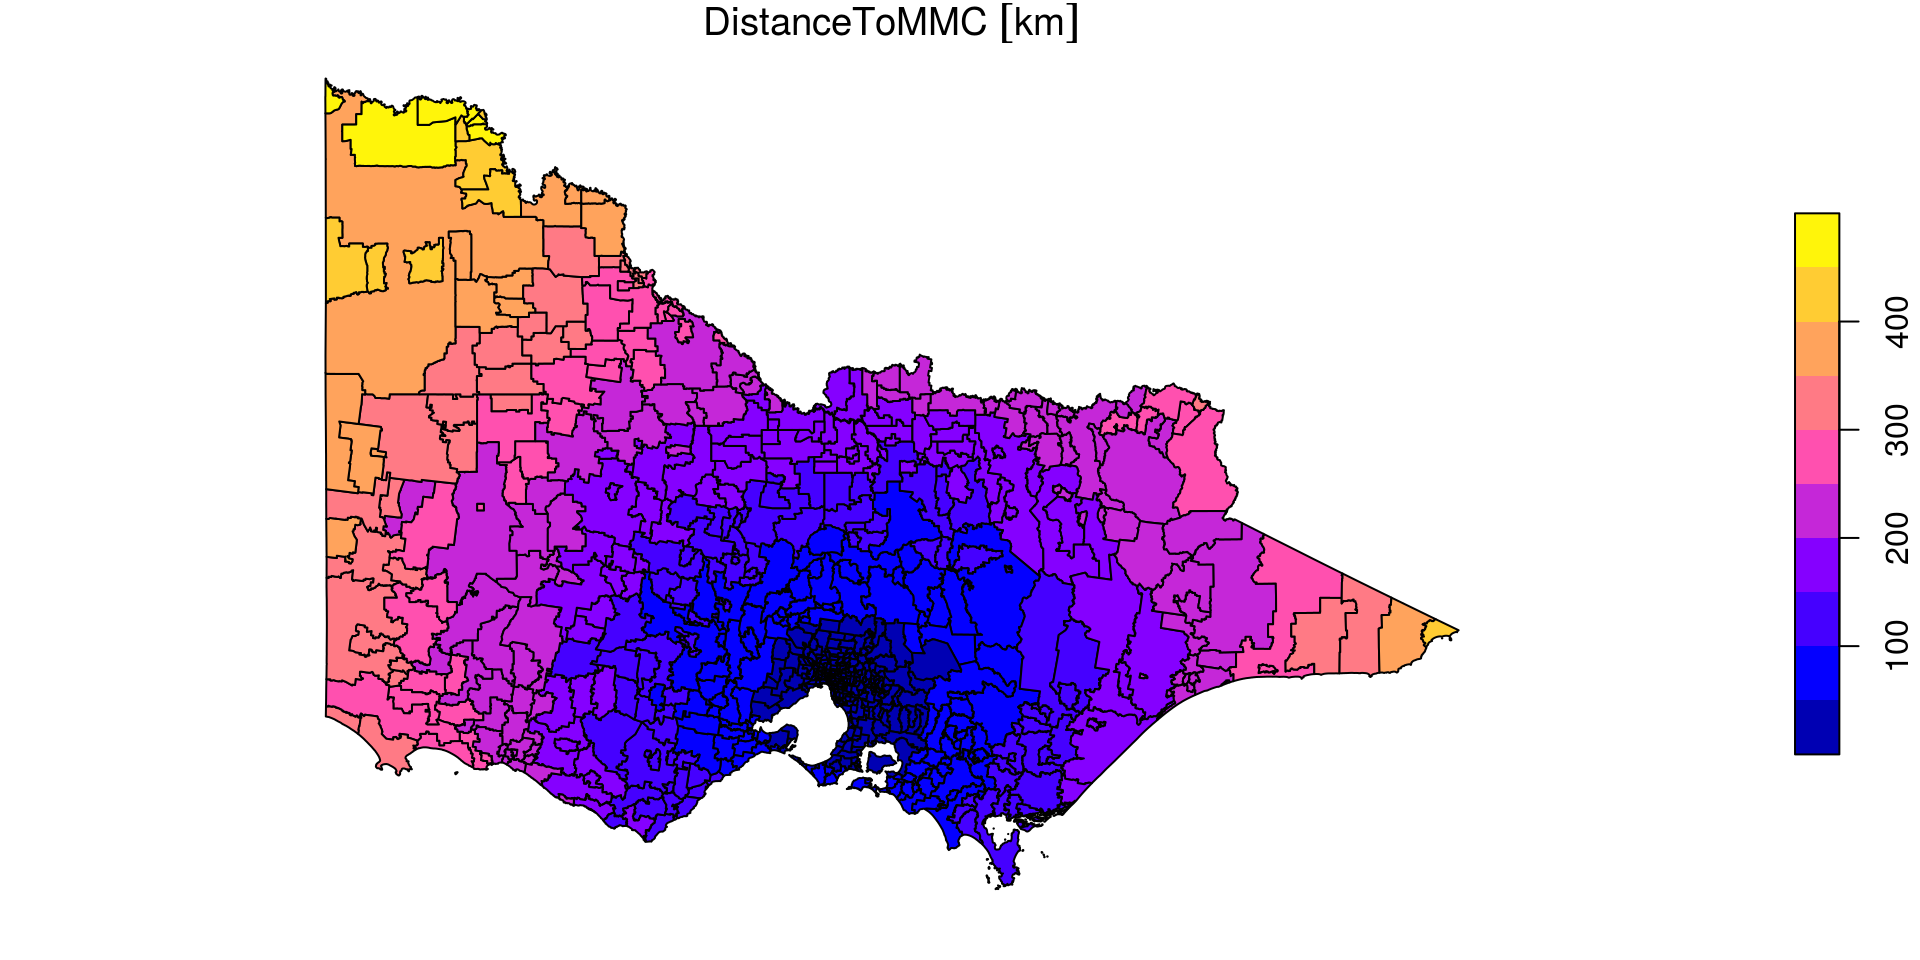
\includegraphics[width=10cm]{distance_mmc.png}
\end{center}
\caption{Visualization of straightline distance calculation from every postcode in the state to Monash Medical Centre. Static visualization created with {\em tmap}}\label{fig:DistanceToMMC}
\end{figure}

\begin{figure}[h!]
\begin{center}
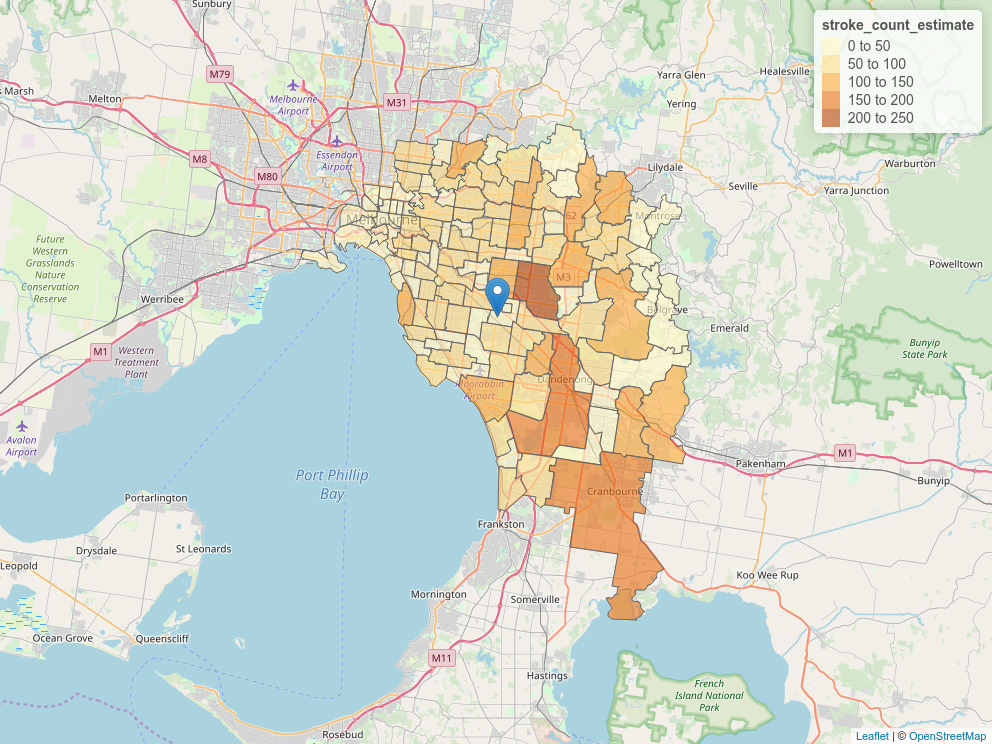
\includegraphics[width=14cm]{choropleth.png}
\end{center}
\caption{Choropleth of stroke case load estimate. Postcodes are coloured according to estimation of stroke cases derived from demographic data. Screenshot of interactive visualization created with {\em tmap}}\label{fig:choropleth}
\end{figure}

\begin{figure}[h!]
\begin{center}
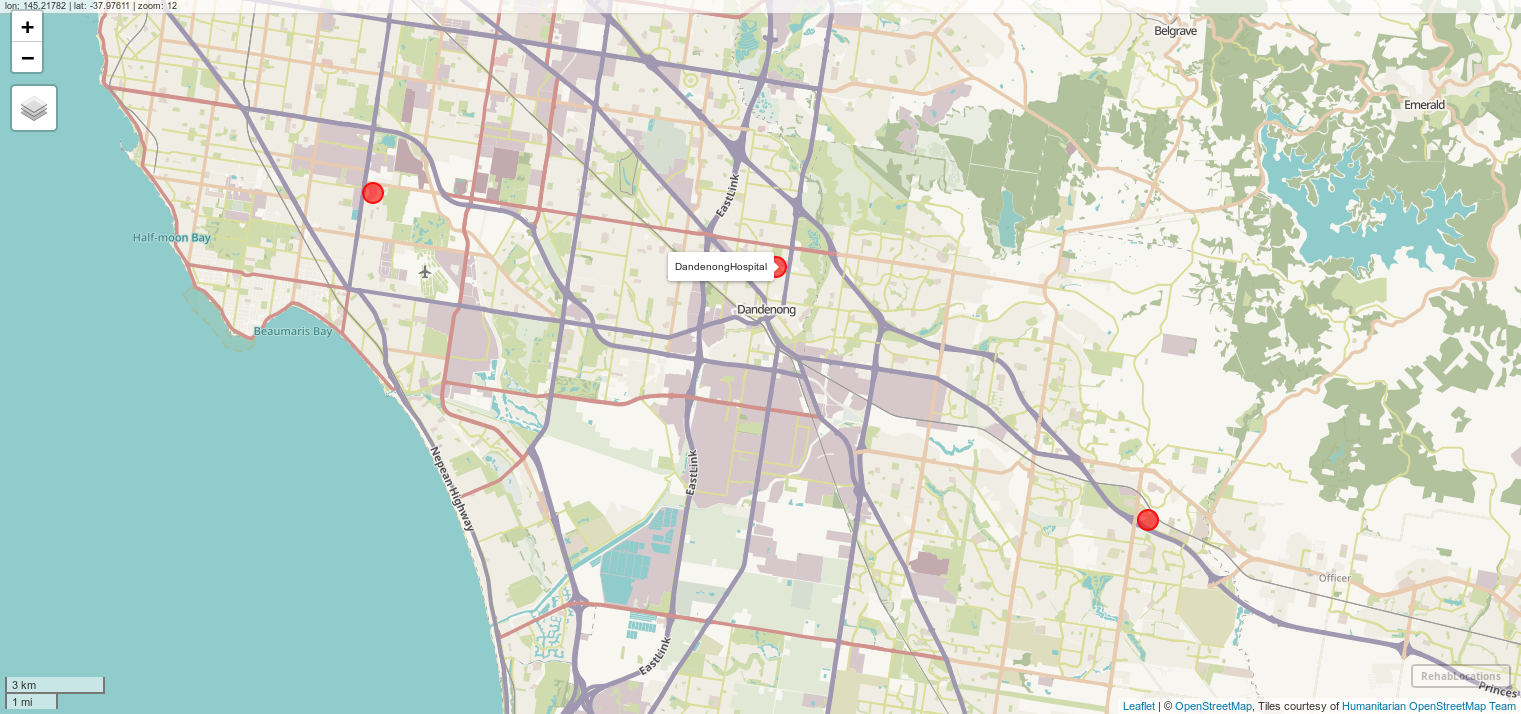
\includegraphics[width=15cm]{map1_mv.png}
\end{center}
\caption{Locations of the three rehabilitation centers determined by geocoding. Screenshot of interactive visualization created with {\em mapview}}\label{fig:RehabCenterLocations}
\end{figure}

\begin{figure}[h!]
\begin{center}
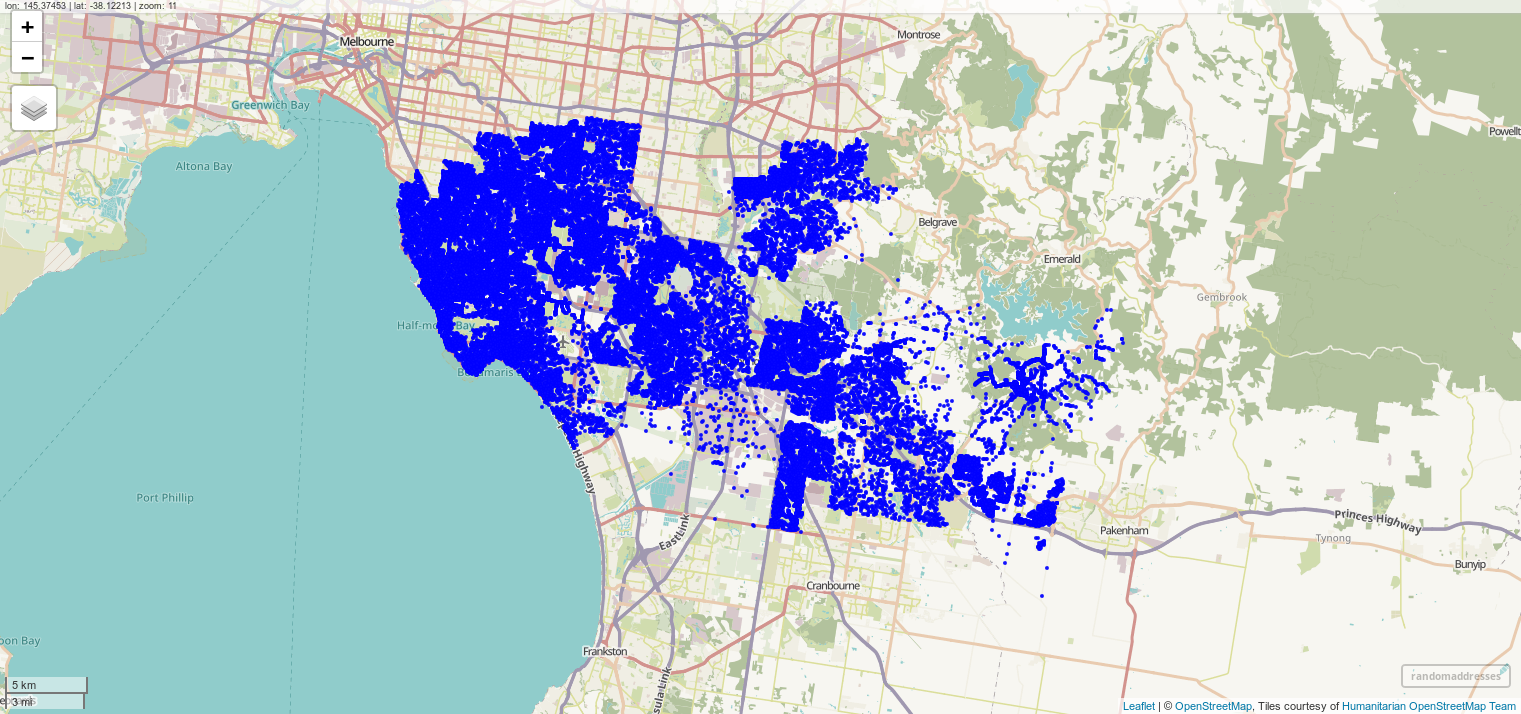
\includegraphics[width=15cm]{map2_mv.png}
\end{center}
\caption{Randomly sampled addresses within the postcodes of interest. 1000 addresses per postcode were sampled, and the differing population density across the postcodes of interest is clearly visible. Screenshot of interactive visualization created with {\em mapview}}\label{fig:RehabCenterRandomAddresses}
\end{figure}

\begin{figure}[h!]
\begin{center}
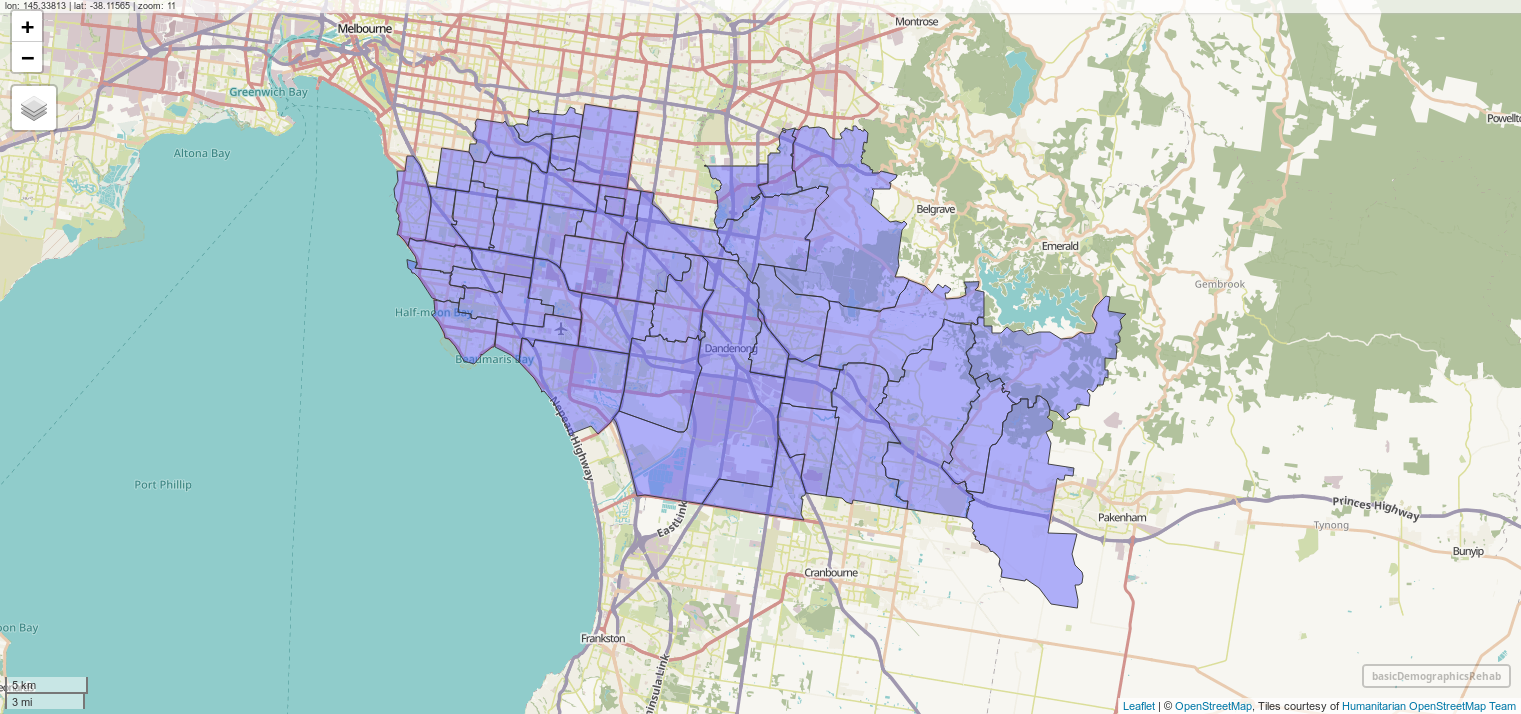
\includegraphics[width=15cm]{map3_mv.png}
\end{center}
\caption{Boundaries of postcodes with centroids within 10km of one of the
  rehabilitation centers. Screenshot of interactive visualization created with {\em mapview}}\label{fig:RehabCenterPostcodes}
\end{figure}

\begin{figure}[h!]
\begin{center}
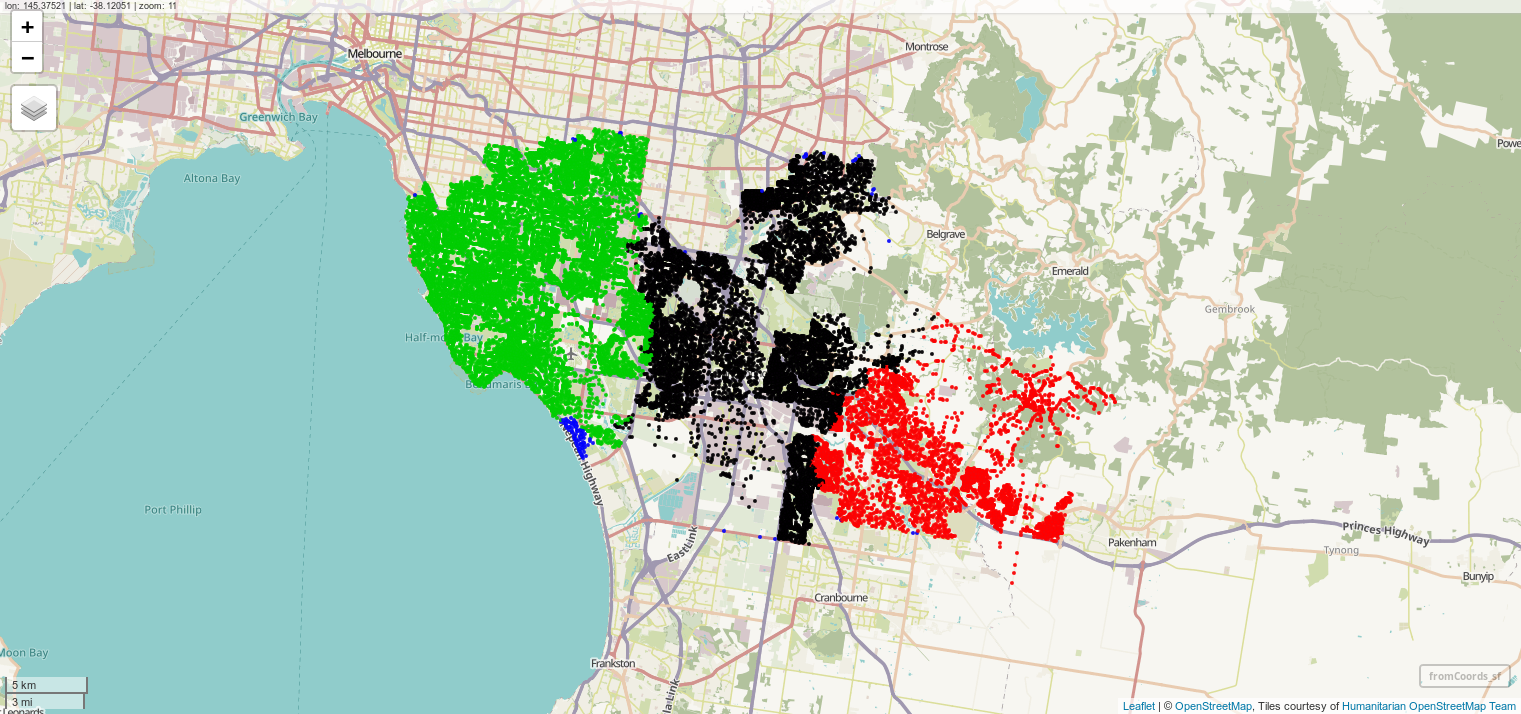
\includegraphics[width=15cm]{map4_mv.png}
\end{center}
\caption{Sampled address colourcoded according to nearest destination, with distance to destination computed through the street network. Screenshot of interactive visualization created with {\em mapview}}\label{fig:RehabCenterAddressCatchments}
\end{figure}

\begin{figure}[h!]
\begin{center}
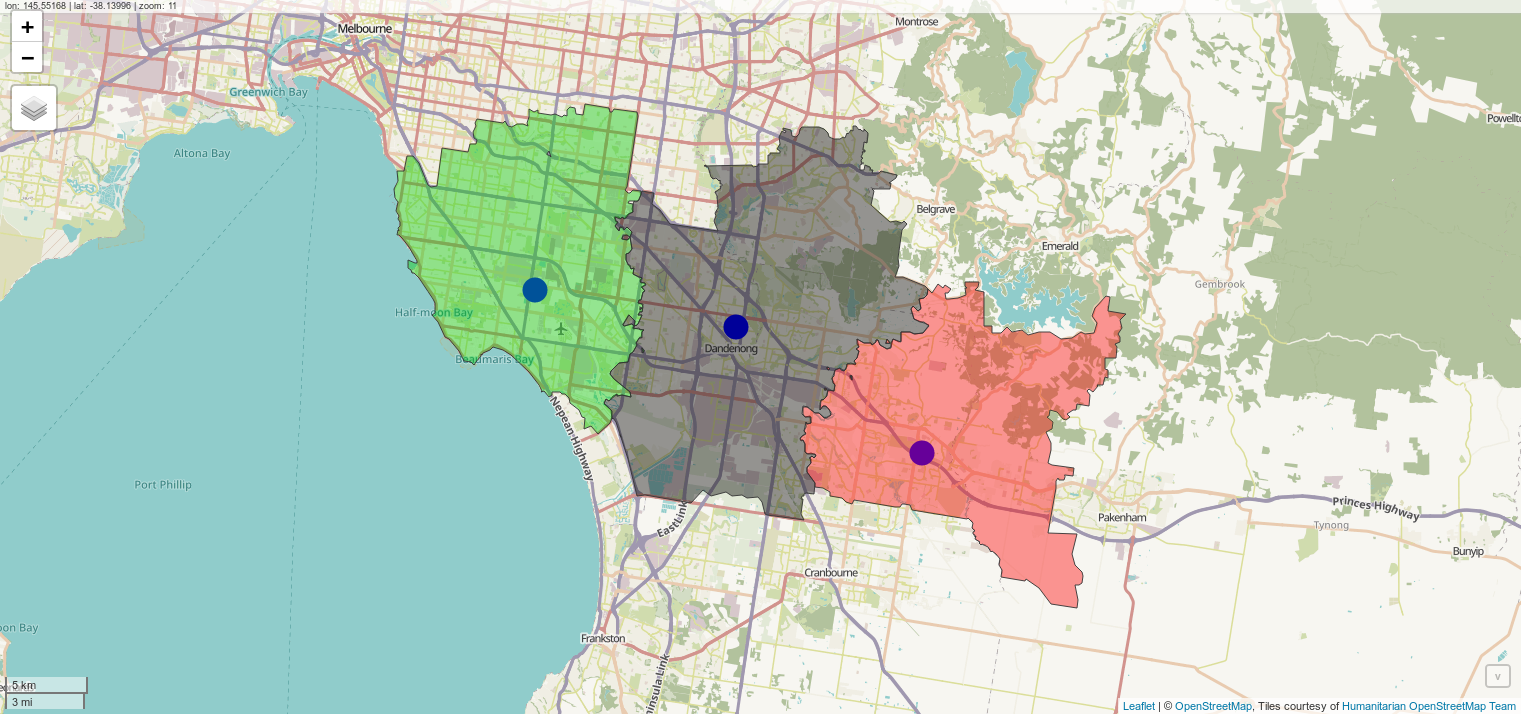
\includegraphics[width=15cm]{map5_mv.png}
\end{center}
\caption{Polygon representation of rehabilitation center catchment zones. Screenshot of interactive visualization created with {\em mapview}}\label{fig:RehabCenterPolyCatchments}
\end{figure}

\begin{figure}[h!]
\begin{center}
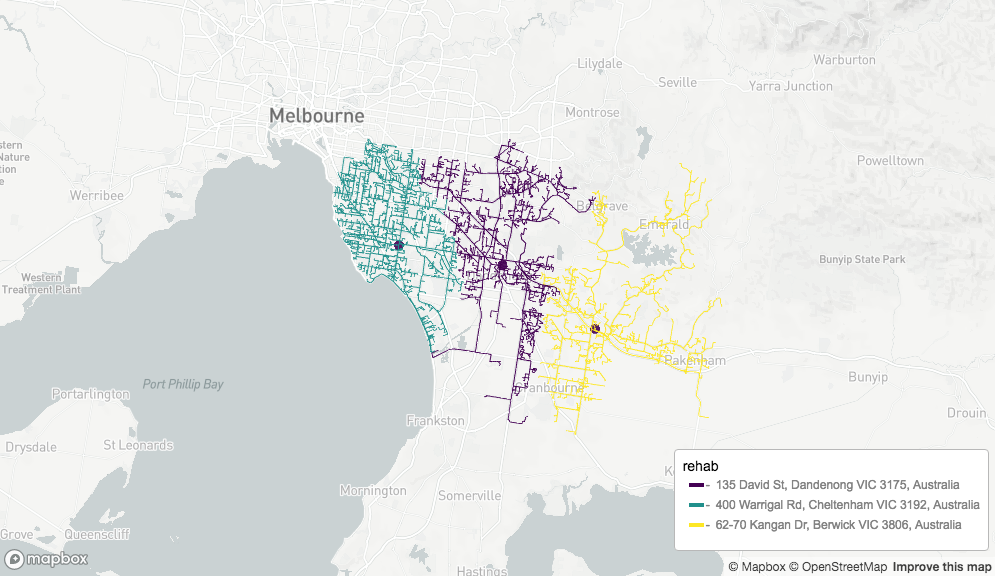
\includegraphics[width=10cm]{nearest_rehab.png}
\end{center}
\caption{Road network-based visualization of catchment zones for rehabilitation centers. Screenshot of interactive visualization created with {\em mapdeck} (API key required)}\label{fig:RehabCenterRoadCatchment}
\end{figure}

\begin{figure}[h!]
\begin{center}
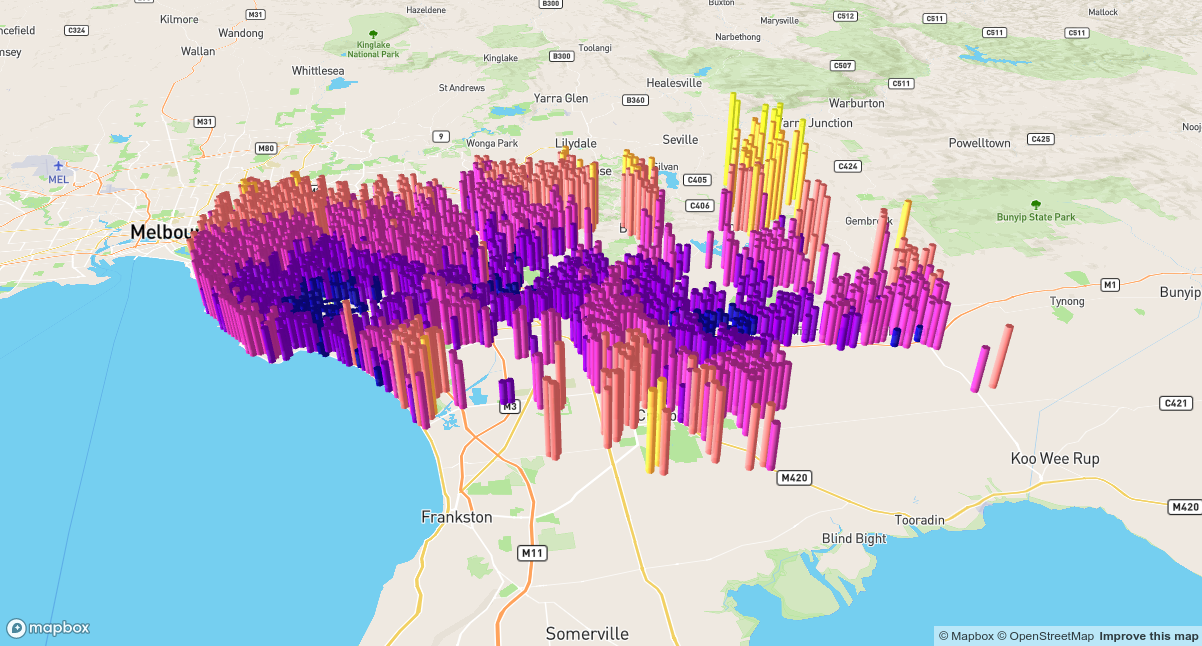
\includegraphics[width=10cm]{directions_all_rehab_mapdeck_hexagons.png}
\end{center}
\caption{Alternative visualization of distances from random addresses to rehabilitation centeres. Screenshot of interactive visualization created with {\em mapdeck} (API key required)}\label{fig:RehabCenterAddressDistanceHex}
\end{figure}

\begin{figure}[h!]
\begin{center}
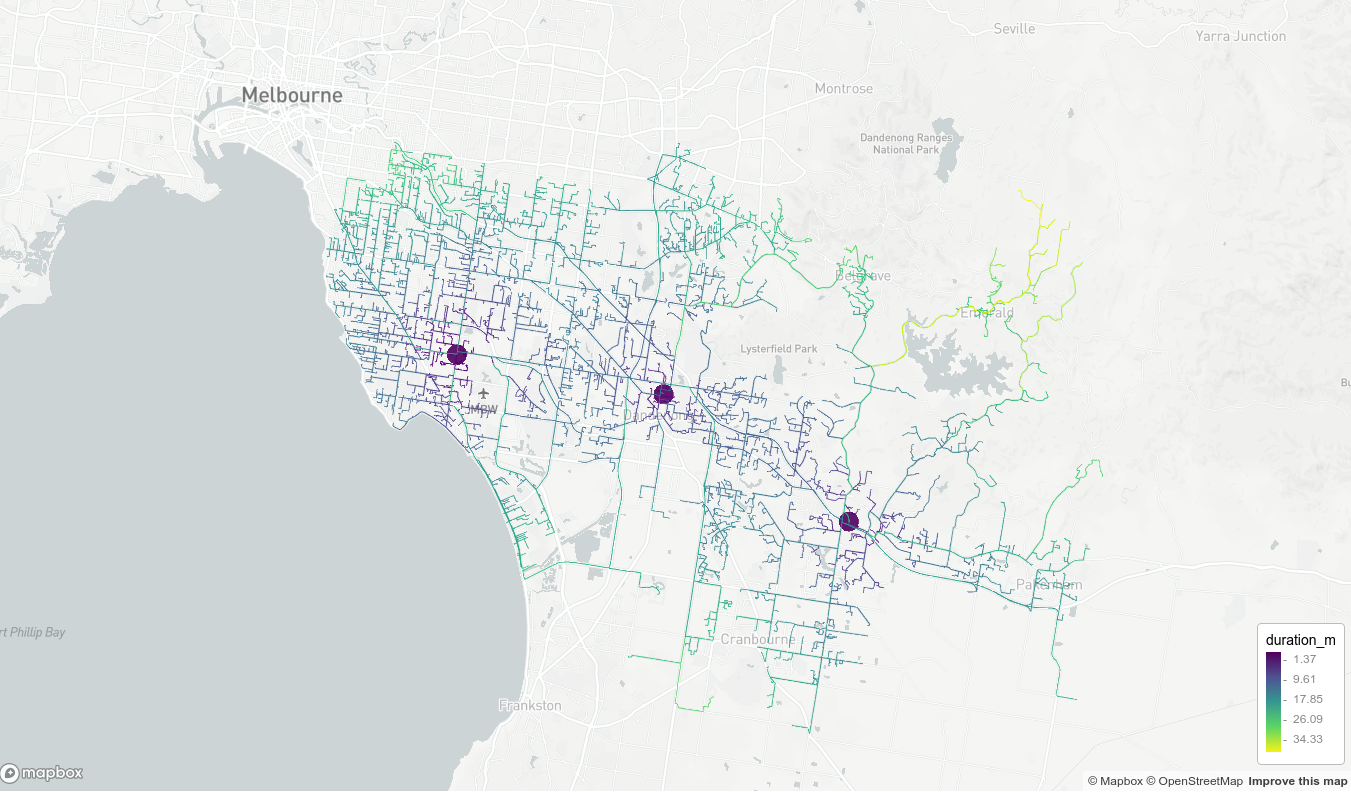
\includegraphics[width=10cm]{duration_all_rehab.png}
\end{center}
\caption{Road network visualization of travel times from random addresses to rehabilitation centeres. Screenshot of interactive visualization created with {\em mapdeck} (API key required)}\label{fig:RehabCenterAddressDistance}
\end{figure}


\end{document}
